%%%%%%%%%% *** The Title %%%%%%%%%%
\title[]{기온\\\small{제3장}}

\begin{frame}[plain] %title page
	\titlepage
\end{frame}


\begin{frame}[plain] %cc page
	\ccpage
\end{frame}


\section{기록: 기온 자료}

\begin{frame}[t]{기본 계산}
	\begin{tabular}{ll}
		\begin{minipage}[t]{0.90\textwidth}
			\begin{itemize}
				\item 일평균 기온(daily mean temperature)
				: 24시간 동안 시간별로 얻어진 자료를 평균하거나 24시간 동안
				의 최고, 최저 기온을 평균한 값
				\item 일교차(daily temperature range)
				: 하루 중 최고 기온과 최저 기온의 차이
				\item 월평균 기온(monthly mean temperature)
				: 한 달의 일평균 기온을 모두 더해 그 달의 날 수로 나눈 값(일평균 기온의 평균값)
				\item 연평균 기온(annual mean temperature)
				: 열두 달의 월평균 기온을 모두 더해 12로 나눈 값(월평균 기온의 평균값)
				\item 연교차(annual temperature range)
				: 가장 더운 달과 가장 추운 달의 월평균 기온의 차이
			\end{itemize}			
		\end{minipage}
		&
	\end{tabular}
\end{frame}




\begin{frame}[t]{등온선(isotherms)}
	\begin{tabular}{ll}
		\begin{minipage}[t]{0.60\textwidth}
			\begin{figure}[t]
				\includegraphics[trim=40 425 190 50, clip, page=93, width=\textwidth]
				{\bookfile}
			\end{figure}
		\end{minipage}	
		&
		\begin{minipage}[t]{0.35\textwidth} \scriptsize
			\begin{itemize}
				\item 같은 온도인 지점을 연결한 선으로, $5 \rm{^\circ}C$ 또는 $10\rm{^\circ}C$ 온도 간격으로 많이 표시함. 
				\item 넓은 지역에 걸친 기온의 분포를 눈으로 쉽게 알 수 있도록 보여주기 위해 사용
				\item 단위 거리에 따른 온도 변화 정도를 온도 경도라고 함.
				\item 등온선 간격이 가까우면 급격한 온도 변화를 나타냄.
				
			\end{itemize}
		\end{minipage}
	\end{tabular}
\end{frame}




\begin{frame}[t]{가장 더운 곳}
	\begin{tabular}{ll}
		\begin{minipage}[t]{0.50\textwidth}	
			\begin{figure}[t]
				\includegraphics[trim=365 445 35 90, clip, page=92, width=\textwidth]
				{\bookfile}
			\end{figure}
		\end{minipage}	
		&
		\begin{minipage}[t]{0.45\textwidth}
			\questionset{여름철 캘리포니아의 데스 밸리에서는 왜 최고 기온이 매우 높게 나타나는가?}
			\solutionset{데스 밸리의 고도는 $–53\rm{~m}$이고, 주위 산의 영향으로 인해 바다로부터 유입되는 수증기가 매우 적고 산을 넘어오는 공기 덩어리의 단열 압축으로 인하여 기온이 높고 깨끗한 하늘을 가진다. \\
			이에 따라 이 지역은 태양 복사가 강하고 강수량이 적어 건조하다. 그러므로 수증기의 증발로 소모되는 에너지가 적기 때문에 대부분의 에너지는 지표면을 데우는 데 사용된다. 이로 인해 이 지역의 기온은 매우 높다.}
		\end{minipage}
	\end{tabular}
\end{frame}







\section{온도는 왜 변화하는가: 온도의 제어}


\begin{frame}[t]{온도 제어 요인}
	\begin{tabular}{ll}
		\begin{minipage}[t]{0.95\textwidth}
			\questionset{온도 제어 요인에는 무엇이 있는가?}
			\solutionset{위도, 육지와 물의 차등 가열, 해류, 고도, 지리적 위치, 알베도 변화 등}
		\end{minipage}	
		&
		\begin{minipage}[t]{\textwidth}
		\end{minipage}
	\end{tabular}
\end{frame}





\begin{frame}[t]{위도}
	\begin{tabular}{ll}
		\begin{minipage}[t]{0.40\textwidth}
			\begin{figure}[t]
				\includegraphics[trim=50 330 320 55, clip, page=94, width=\textwidth]
				{\bookfile}
			\end{figure}
		\end{minipage}	
		&
		\begin{minipage}[t]{0.55\textwidth}
			\begin{itemize}
				\item 위도에 따라 태양각과 낮의 길이가 다르다
				\item 그러므로 기본적으로 저위도에서는 온도가 높고, 고위도에서는 온도가 낮다
				\item 주어진 위도에서 계절별 온도 변동은 태양 적위의 변화에 의해 발생한다.				
			\end{itemize}
		\end{minipage}
	\end{tabular}
\end{frame}



\begin{frame}[t]{육지와 물의 차등 가열}
	\begin{tabular}{ll}
		\begin{minipage}[t]{0.35\textwidth}
			\begin{figure}[t]
				\includegraphics[trim=350 35 50 355, clip, page=94, width=\textwidth]
				{\bookfile}
			\end{figure}
		\end{minipage}	
		&
		\begin{minipage}[t]{0.6\textwidth}\scriptsize
			\begin{itemize}
				\item 그림처럼 가열될 때는 육지가 바다보다 빠르게 가열되어 육지의 온도가 해수면의 온도보다 더 높음.
				\item 반대로 냉각될 때는 육지가 바다보다 빠르게 냉각되어 육지의 온도가 해수면의 온도보다 더 낮음.
				\item 기온의 변동은 육지로 덮여 있는 지역이 물로 덮여 있는 지역보다 더 크다.
			\end{itemize}
				\questionset {육지와 물의 가열과 냉각이 다르게 일어나는 이유를 설명하시오.}
				\solutionset{1)물의 큰 유동성 : 물이 가열되면 대류에 의해 깊은 지역까지 열을 분배하지만, 땅은 유체가 아니므로 혼합이 일어나지 않는다. \\
				2) 불투명한 지표면, 투명한 물 : 지표면은 불투명하여 오직 표면에서만 태양 복사가 흡수되지만, 물은 지표면보다는 태양 복사를 더 투과 시키므로 수 미터의 깊이까지 태양 복사가 전달된다.\\ 
				3) 물의 육지의 비열 차이 : 물의 비열이 육지의 비열 보다 3배 이상 크다.\\
				4) 수면에서의 증발 : 물의 기화열, 승화열이 매우 크고, 수면에서의 증발이 지면에서의 증발보다 더 많은 에너지를 필요로 한다.}
		\end{minipage}
	\end{tabular}
\end{frame}



\begin{frame}[t]{육지와 물의 차등 가열}
	\begin{tabular}{ll}
		\begin{minipage}[t]{0.45\textwidth}
			\begin{figure}[t]
				\includegraphics[trim=340 410 40 60, clip, page=95, width=\textwidth]
				{\bookfile}
			\end{figure}
		\end{minipage}	
		&
		\begin{minipage}[t]{0.5\textwidth}
			\questionset{제시된 그래프의 두 지역의 연교차를 비교하고, 그 이유를 설명하시오.}
			\solutionset{같은 위도에 위치하여 유사한 태양각과 낮의 길이를 가지고 있지만 연간 온도변화 폭은 다르다 \\
			육지의 영향을 받는 위니펙의 연간 기온 변화가  바다의 영향을 받는 벤쿠버 보다 크다.}
		\end{minipage}
	\end{tabular}
\end{frame}



\begin{frame}[t]{육지와 물의 차등 가열}
	\begin{tabular}{ll}
		\begin{minipage}[t]{0.6\textwidth}
			\begin{figure}[t]
				\includegraphics[trim=50 450 120 50, clip, page=96, width=0.9\textwidth]
				{\bookfile}
			\end{figure}
		\end{minipage}	
		&
		\begin{minipage}[t]{0.35\textwidth}
			\begin{figure}[t]
			\includegraphics[trim=40 30 350 580, clip, page=96, width=\textwidth]
			{\bookfile}
		\end{figure}
		\end{minipage}
	\end{tabular}
		\newline
		
		\questionset{위의 그림과 표를 참고하여 남반구와 북반구의 연교차를 비교하여 설명하시오.}
		\solutionset{남반구는 81\% 해양, 19\% 육지로 구성, 북반구는 61\% 해양, 39\% 육지로 구성 \\
		⇒ 해양이 지배적인 남반구에서 기온의 연교차가 작다}
\end{frame}





\begin{frame}[t]{해류}
	\begin{tabular}{ll}
		\begin{minipage}[t]{0.90\textwidth}
			\begin{figure}[t]
				\includegraphics[trim=10 430 40 62, clip, page=97, width=0.85\textwidth]
				{\bookfile}
			\end{figure}
		\end{minipage}	
		&
		\begin{minipage}[t]{0.05\textwidth}

		\end{minipage}
	\end{tabular}

		\begin{itemize} \scriptsize 
			\item 난류와 한류는 해안과 인접한 지역의 겨울과 여름철 기온에 큰 영향
			\item 난류의 효과는 겨울에 잘 나타나며, 한류의 효과는 여름에 잘 나타남.				
		\end{itemize}
\end{frame}





\begin{frame}[t]{해류}
	\begin{tabular}{ll}
		\begin{minipage}[t]{0.475\textwidth}
			\begin{figure}[t]
				\includegraphics[trim=140 550 300 60, clip, page=97, width=0.85\textwidth]
				{\bookfile}
			\end{figure}
		
		\begin{itemize} \scriptsize 
			\item 위도가 $52 \rm{{^\circ}N}$인 베를린과 $40 \rm{{^\circ}N}$인 뉴욕의 1월 평균 기온 비슷
		\end{itemize}
		\end{minipage}	
		&
		\begin{minipage}[t]{0.475\textwidth}
			\begin{figure}[t]
				\includegraphics[trim=220 480 230 140, clip, page=97, width=0.85\textwidth]
				{\bookfile}
			\end{figure}
		
		\begin{itemize} \scriptsize 
			\item 위도가 $23 \rm{{^\circ}S}$인 윌비스베이는 위도가 $29 \rm{{^\circ}S}$인 더반보다 여름철에 더 서늘함				
		\end{itemize}
		\end{minipage}
	\end{tabular}
	

\end{frame}






\begin{frame}[t]{해류}
	\begin{tabular}{ll}
		\begin{minipage}[t]{0.50\textwidth}
			\begin{figure}[t]
				\includegraphics[trim=330 30 40 465, clip, page=97, width=\textwidth]
				{\bookfile}
			\end{figure}
		\end{minipage}	
		&
		\begin{minipage}[t]{0.45\textwidth}
			\questionset{제시된 그래프의 두 지역의 여름 기온을 비교하고, 그 이유를 설명하시오.}
			\solutionset{두 지역은 해수면 정도 고도의 연안 도시인데, 적도에 더 가까운 아리카의 여름 기온이 리우데자네이루보다 낮게 나타난다. \\
			아리카는 한류의 영향을 받는 지역이며, 리우데자네이루는 난류의 영향을 받는 지역이기 때문이다.}
		\end{minipage}
	\end{tabular}
\end{frame}




\begin{frame}[t]{고도}
	\begin{tabular}{ll}
		\begin{minipage}[t]{0.450\textwidth}
			\begin{figure}[t]
				\includegraphics[trim=350 30 40 460, clip, page=98, width=\textwidth]
				{\bookfile}
			\end{figure}
		\end{minipage}	
		&
		\begin{minipage}[t]{0.5\textwidth}
			\begin{itemize} \scriptsize 
				\item 위도가 비슷하더라도 고도가 높은 지역의 기온이 낮고 연교차도 작다.
				\item 위도가 비슷하더라도 고도가 높은 지역의 일교차가 더 크다.
			\end{itemize}			
			
			\questionset{고도가 높은 지역의 일교차가 큰 이유를 설명하시오.}
			\solutionset{고도가 증가함에 따라 대기 압력과 밀도도 감소한다. 고도가 올라갈수록 밀도가 감소하므로 특정 고도 위의 대기는 태양복사 중 적은 양만 흡수, 반사, 산란한다. 즉, 고도가 증가하면 주간 태양복사 강도가 증가하여 상대적으로 빠르고 강한 가열이 이루어지고, 반대로 야간에는 냉각이 급속히 이루어진다.}
		\end{minipage}
	\end{tabular}
\end{frame}




\begin{frame}[t]{지리적 분포}
	\begin{tabular}{ll}
		\begin{minipage}[t]{0.50\textwidth}
			\begin{figure}[t]
				\includegraphics[trim=35 50 350 470, clip, page=99, width=\textwidth]
				{\bookfile}
			\end{figure}
		\end{minipage}	
		&
		\begin{minipage}[t]{0.45\textwidth}
			\begin{itemize} \scriptsize 
				\item 해양에서 부는 바람의 영향을 받는 지역(풍상측)이, 육지에서 부는 바람의 영향을 받는 지역(풍하측)에 있는 지역보다 연교차가 작게 나타남
				\item 편서풍 대의 대륙 서안 기후(풍상측), 대륙 동안 기후(풍하측)
			\end{itemize}	
		\end{minipage}
	\end{tabular}	
\end{frame}




\begin{frame}[t]{지리적 분포}
	\begin{tabular}{ll}
		\begin{minipage}[t]{0.50\textwidth}
			\begin{figure}[t]
				\includegraphics[trim=330 450 40 50, clip, page=99, width=\textwidth]
				{\bookfile}
			\end{figure}
		\end{minipage}	
		&
		\begin{minipage}[t]{0.45\textwidth}
		\questionset{시애틀과 스포캔은 불과 $360 \rm{~km}$밖에 떨어져 있지 않지만 연교차는 매우 다르다. 그 이유를 설명하시오.}
		\solutionset{워싱턴 주의 시애틀과 스포캔은 캐스캐이드 산맥이 두 도시를 분리한다. 결론적으로 시애틀은 바다의 영향을 많이 받는데 비해 스포캔은 전형적인 대륙의 영향을 나타낸다.}
		\end{minipage}
	\end{tabular}
			
\end{frame}



\begin{frame}[t]{알베도 변화}
	\begin{tabular}{ll}
		\begin{minipage}[t]{0.450\textwidth}
			\begin{figure}[t]
				\includegraphics[trim=50 420 340 50, clip, page=100, width=\textwidth]
				{\bookfile}
			\end{figure}
		\end{minipage}	
		&
		\begin{minipage}[t]{0.5\textwidth}
			\begin{itemize} \scriptsize 
				\item 운량은 일 최고기온을 낮추고, 최저기온을 높여 일교차를 작게 함.
				\item 운량이 많으면 알베도가 증가하여 태양복사를 
				반사시켜 최고 기온을 낮춤
				\item 운량이 많으면 야간에는 지구 복사를 흡수하고, 
				일부를 지표로 방출함. 
				\item 그러므로 구름 낀 날 야간의 기온이 맑은 날보다 높음.
				
			\end{itemize}			
		\end{minipage}
	\end{tabular}
	
\end{frame}



\begin{frame}[t]{알베도 영향}
	\begin{tabular}{ll}
		\begin{minipage}[t]{0.450\textwidth}
			\begin{figure}[t]
				\includegraphics[trim=350 390 30 50, clip, page=100, width=0.9\textwidth]
				{\bookfile}
			\end{figure}
		\end{minipage}	
		&
		\begin{minipage}[t]{0.5\textwidth}
			\begin{itemize} \scriptsize 
				\item 운량은 월평균 기온에 영향을 미침. 
				\item 예를 들어, 여름에는 우기이므로 구름의 양이 많아져서 태양복사의 지표 입사를 줄이는 반면, 봄에는 건기이므로 하늘이 상대적으로 맑아 태양복사가 지표로 도달하는 양이 많아져서 최고 기온이 4, 5월임.
			\end{itemize}			
		\end{minipage}
	\end{tabular}
	
\end{frame}



\begin{frame}[t]{알베도 영향}
	\begin{tabular}{ll}
		\begin{minipage}[t]{0.50\textwidth}
			\begin{figure}[t]
				\includegraphics[trim=350 0 30 550, clip, page=100, width=\textwidth]
				{\bookfile}
			\end{figure}
		\end{minipage}	
		&
		\begin{minipage}[t]{0.45\textwidth}
			\begin{itemize} \scriptsize 
				\item 지표의 눈과 얼음은 알베도를 높여서 최고 기온은 낮춤.
				\item 해빙의 양의 증가는 알베도를 낮춰서 북극의 온도를 높임.
			\end{itemize}			
		\end{minipage}
	\end{tabular}
	
\end{frame}








\section{전 세계 기온의 분포}


\begin{frame}[t]{1월의 기온 분포}
	\begin{tabular}{ll}
		\begin{minipage}[t]{0.90\textwidth}
			\begin{figure}[t]
				\includegraphics[trim=40 20 60 455, clip, page=101, width=0.8\textwidth]
				{\bookfile}
			\end{figure}
		\end{minipage}	
		&
		\begin{minipage}[t]{0.05\textwidth}
		\end{minipage}
	\end{tabular}	

		\questionset {제시된 그림은 1월의 세계 온도분포를 나타낸 것이다. 등온선이 일반적으로 동-서로 평행한 패턴을 보이는 이유는 무엇인가?}
		\solutionset {위도에 따라 태양의 남중고도와 낮의 길이가 달라져서 태양 복사 에너지가 달라지기 때문에, 적도에서 극으로 갈수록 온도는 감소한다.}		
		
\end{frame}



\begin{frame}[t]{7월의 기온 분포}
	\begin{tabular}{ll}
		\begin{minipage}[t]{0.90\textwidth}
			\begin{figure}[t]
				\includegraphics[trim=40 20 50 455, clip, page=102, width=0.8\textwidth]
				{\bookfile}
			\end{figure}
		\end{minipage}	
		&
		\begin{minipage}[t]{0.05\textwidth}
		
		\end{minipage}
	\end{tabular}
	
		\questionset {제시된 그림은 7월의 세계 온도분포를 나타낸 것이다. 북반구 여름철, 대륙에 
			걸친 등온선은 어느 쪽으로 구부러져 있는지 그 이유와 함께 설명하시오. }
		\solutionset {북반구 여름철에는 물의 비열이 땅의 3배 정도이므로 해양의 온도가 대륙의 온도에 비해 쉽게 오르지 않아서, 대륙에서는 극쪽으로 해양의 경계에서는 적도 쪽으로 구부러져 있다.}	
		
\end{frame}




\begin{frame}[t]{세계의 기온 분포}
	\begin{tabular}{ll}
		\begin{minipage}[t]{0.4750\textwidth}
			\begin{figure}[t]
				\includegraphics[trim=40 20 60 455, clip, page=101, width=\textwidth]
				{\bookfile}
			\end{figure}
		\end{minipage}	
		&
		\begin{minipage}[t]{0.475\textwidth}
			\begin{figure}[t]
			\includegraphics[trim=40 20 50 455, clip, page=102, width=\textwidth]
			{\bookfile}
		\end{figure}	
		\end{minipage}
	\end{tabular}
	
	\questionset {제시된 그림은 1월과 7월의 세계 온도분포를 나타낸 것이다. 등온선이 해류의 존재를 어떻게 보여주는지 설명하시오. }
	\solutionset {난류가 흐르는 곳은 등온선이 극 쪽으로 굽어지며, 한류가 흐르는 곳은 등온선이 적도 쪽으로 굽어지게 한다. 그러므로 난류가 흐르는 지역의 온도는 같은 위도 지역보다 온도가 높고, 한류가 흐르는 지역의 온도는 같은 위도 지역보다 온도가 낮다. \newline}
	
	\questionset{제시된 그림은 1월과 7월의 세계 온도분포를 나타낸 것이다. 등온선이 남반구보다 북반구에서 더 불규칙한 이유를 설명하시오.}
	\solutionset{북반구에는 온도의 변화가 점진적으로 일어나는 해양보다 대륙이 더 많이 분포되어 있기 때문이다.}
	
\end{frame}




\begin{frame}[t]{연교차}
	\begin{tabular}{ll}
		\begin{minipage}[t]{0.90\textwidth}
			\begin{figure}[t]
				\includegraphics[trim=40 405 60 60, clip, page=103, width=0.8\textwidth]
				{\bookfile}
			\end{figure}
		\end{minipage}	
		&
		\begin{minipage}[t]{0.05\textwidth}
		\end{minipage}
	\end{tabular}
	
	\questionset{지구에서 연교차가 가장 큰 곳은 어느 지역인가? 이 지역에서 연교차가 큰 이유는 무엇인가?}
	\solutionset{시베리아 지역이다. 해양으로부터 영향을 적게 받는 대륙의 중심부 지역이고, 겨울철에 온도가 매우 낮기 때문이다.}
	
\end{frame}



\begin{frame}[t]{위도별 연교차}
	\begin{tabular}{ll}
		\begin{minipage}[t]{0.40\textwidth}
			\begin{figure}[t]
				\includegraphics[trim=50 250 360 260, clip, page=104, width=\textwidth]
				{\bookfile}
			\end{figure}
		\end{minipage}	
		&
		\begin{minipage}[t]{0.55\textwidth}
			\begin{figure}[t]
				\includegraphics[trim=320 245 30 305, clip, page=104, width=0.8\textwidth]
				{\bookfile}
			\end{figure}
			
			\questionset{적도 근처에서의 연교차와 고위도 지방에서의 연교차를 비교하면 어떻게 되는가?}
			\solutionset{적도 근처는 계절에 따른 태양 고도 차이에 의한 복사량의 차이가 적기 때문에 고위도 지방에 비해 연교차가 작다.}
			
		\end{minipage}
	\end{tabular}
	
	
\end{frame}




\section{기온 주기}

\begin{frame}[t]{기온 일주기}
	\begin{tabular}{ll}
		\begin{minipage}[t]{0.90\textwidth}
			\begin{figure}[t]
				\includegraphics[trim=50 40 80 570, clip, page=104, width=\textwidth]
				{\bookfile}
			\end{figure}
		\end{minipage}	
		&
		\begin{minipage}[t]{0.05\textwidth}
		\end{minipage}
	\end{tabular}

		\questionset{일교차가 큰 날은 어떤 날인가?}
		\solutionset{맑은 날일수록 일교차가 크다. \newline}
		
		\questionset{자동기상관측시스템 (AWS, Automatic Weather Station) 자료를 이용하여 아래와 같이 기온 변화 그래프를 그려보자.}
		\solutionset{실험 시간에 Python 으로}		

\end{frame}



\begin{frame}[t]{일 최저기온}
	\begin{tabular}{ll}
		\begin{minipage}[t]{0.90\textwidth}
			\begin{figure}[t]
				\includegraphics[trim=30 455 50 50, clip, page=105, width=0.8\textwidth]
				{\bookfile}
			\end{figure}
		\end{minipage}	
		&
		\begin{minipage}[t]{0.05\textwidth}
		\end{minipage}
	\end{tabular}
	
	\questionset{하루 중 기온이 가장 낮은 때는 언제인가? 그리고 그 이유는 무엇인가?}
	\solutionset{하루 중 기온이 가장 낮을 때는 해뜨기 직전이다. 해뜨기 전까지 밤새도록 지표면 근처의 공기가 복사 냉각되기 때문에 새벽에 아래 그림과 같이 서리나 안개가 형성된다.}				
\end{frame}



\begin{frame}[t]{기온 일주기}
	\begin{tabular}{ll}
		\begin{minipage}[t]{0.45\textwidth}
			\begin{figure}[t]
				\includegraphics[trim=40 40 350 410, clip, page=105, width=\textwidth]
				{\bookfile}
			\end{figure}
		\end{minipage}	
		&
		\begin{minipage}[t]{0.5\textwidth}
			\questionset{입사되는 태양 복사의 강도가 정오 시간에 강하지만, 하루 중 가장 따뜻한 시간은 오후 3시 경이다. 그 이유를 설명하시오.}
			\solutionset{태양 복사 에너지는 태양의 고도가 가장 높은 정오에 최대이지만, 지표가 흡수한 에너지를 다시 지구복사의 형태로 대기 중으로 전달하는 데에는 시간이 필요하므로 지구 복사 에너지 최대 지점은 오후 시간이다. \\
			흡수하는 태양복사에너지가 방출하는 지구 복사 에너지를 초과하는 한 지표는 계속 가열되므로, 오후에 하루 중 가장 따뜻한 시점이 존재한다.}				
		\end{minipage}
	\end{tabular}
\end{frame}



\begin{frame}[t]{일교차의 변화}
	\begin{tabular}{ll}
		\begin{minipage}[t]{0.90\textwidth}
			\questionset{일교차의 크기는 지역적 요소와 국지적 일기 조건에 따라 상당히 변할 수 있다. 이러한 변화를 유발하는 요인을 네 가지 기술하시오.}
			\solutionset{1) 지역에 따라 태양의 고도각의 변화가 차이가 난다. 태양의 고도각이 큰 곳은 낮 동안 온도변화가 크다. 반면 극지방과 같이 태양의 고도각이 작은 곳은 낮 동안의 온도 변화가 작아서 일교차가 작다.\\
			2) 해양은 비열이 크고 열수송이 활발히 일어나기 때문에 하루 동안 해양의 온도변화는 $1 \rm{{^\circ}C}$보다 작은 편이다. 따라서 바람이 불어오는 쪽의 해안에 위치한 곳은 온도변화가 완만하다.\\
			3) 구름이 많아 흐린 날의 낮에는 태양 복사 에너지의 흡수가 적어 가열이 적고, 밤에는 지구 복사 에너지를 흡수하기 때문에 냉각도 적다. 따라서 흐린 날의 경우 온도 변화가 크지 않다. \\
			4) 대기의 수증기는 장파 복사를 흡수하는 경향이 있으므로 습한 날은 건조한 날에 비해 상대적으로 온도 변화가 크지 않다.}				
		\end{minipage}	
		&
		\begin{minipage}[t]{0.05\textwidth}
		\end{minipage}
	\end{tabular}

\end{frame}


\begin{frame}[t]{인공위성에서 관측한 지표면 온도}
	\begin{tabular}{ll}
		\begin{minipage}[t]{0.90\textwidth}
			\begin{figure}[t]
				\includegraphics[trim=40 440 340 178, clip, page=106, width=0.7\textwidth]
					{\bookfile}
			\end{figure}	
		\end{minipage}	
		&
		\begin{minipage}[t]{0.05\textwidth}
		\end{minipage}
	\end{tabular}
	
		\questionset{테라와 아쿠아 위성에 탑재되어 있는 MODIS를 이용하여 얻은 2월의 평균 지표면 온도를 나타낸 그림에서 흰색 화살표 지점의 대략적인 온도는 얼마인가? 이러한 차이가 나타나는 이유는 무엇일까?}
		\solutionset{-10 도, +10도 정도이다. 이러한 차이는 여러 요인에 의해 나타나겠지만, 주된 요인은 난류의 영향으로 추측된다.}	
\end{frame}



\begin{frame}[t]{도시 열섬(urban heat island)}
	\begin{tabular}{ll}
		\begin{minipage}[t]{0.450\textwidth}
			\begin{figure}[t]
				\includegraphics[trim=50 415 360 60, clip, page=108, width=0.9\textwidth]
				{\bookfile}
			\end{figure}	
		\end{minipage}	
		&
		\begin{minipage}[t]{0.5\textwidth}
			\questionset{도시 열섬 현상에 기여하는 세 가지 요인을 설명하시오.}
			\solutionset{1) 낮 동안 콘크리트, 아스팔트, 높은 빌딩이 태양 복사 에너지를 흡수하여 저장하고 있다가 야간에도 내어 놓기 때문에\\
				2) 시골에 비해 물의 투수율이 적어서 빗물이 빠르게 흐르게 되어 수분 증발량이 크게 줄어들면서, 수증기의 증발에 사용되던 열이 지표면 온도를 증가시키는데 사용되기 때문에\\
				3) 냉난방, 발전소, 공장, 자동차 등으로부터 에너지가 방출되며, 대기 중 에어로졸이 지표에서 방출된 지구 복사 에너지를 일부 흡수하기 때문에}	
		\end{minipage}
	\end{tabular}
\end{frame}



\begin{frame}[t]{도시 열섬(urban heat island)}
	\begin{tabular}{ll}
		\begin{minipage}[t]{0.450\textwidth}
			\begin{figure}[t]
				\includegraphics[trim=220 350 50 80, clip, page=107, width=\textwidth]
				{\bookfile}
			\end{figure}	
		\end{minipage}	
		&
		\begin{minipage}[t]{0.5\textwidth}
			\questionset{도시 열섬 현상을 해결할 수 있는 방안에는 무엇이 있을까?}
			\solutionset{\begin{figure}[t]
					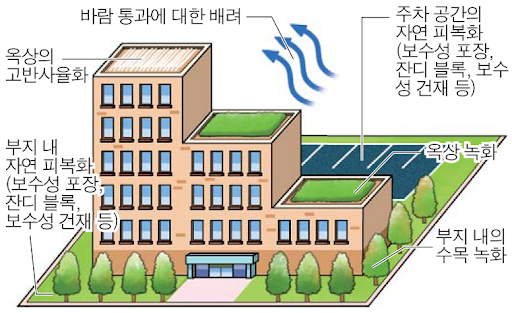
\includegraphics[width=\textwidth]
					{./images/solution_heat_island}
			\end{figure}}	
		\end{minipage}
	\end{tabular}
\end{frame}







\section{온도 측정}



\begin{frame}[t]{액체 온도계}
	\begin{tabular}{ll}
		\begin{minipage}[t]{0.45\textwidth}
			\begin{figure}[t]
				\includegraphics[trim=40 390 350 60, clip, page=109, width=0.9\textwidth]
				{\bookfile}
			\end{figure}
			
		\end{minipage}	
		&
		\begin{minipage}[t]{0.5\textwidth}

			{\scriptsize 액체 온도계 (수은, 알코올 온도계) : 온도가 상승하면 유체의 분자가 더 활동적이고 팽창한다는 원리를 이용}
			
		\end{minipage}	

	\end{tabular}
\end{frame}




\begin{frame}[t]{최고/최저 온도계}
	\begin{tabular}{ll}
		\begin{minipage}[t]{0.90\textwidth}
			\begin{figure}[t]
				\includegraphics[trim=40 40 270 555, clip, page=109, width=0.7\textwidth]
				{\bookfile}
			\end{figure}
		\end{minipage}	
		&
		\begin{minipage}[t]{0.05\textwidth}
			
		\end{minipage}	
	\end{tabular}
	\begin{itemize} \scriptsize 
		\item 최고 온도계: 수은을 이용하는 경우가 많으며, 온도가 내려가면 협착점(제어관)에서 수은이 되돌아가는 것을 방해하여 최고 온도가 기록되게 한다.
		\item 최저 온도계: 밀도가 낮은 알코올을 이용하고 작은 덤벨 모양의 지표가 있어 온도가 낮아지면 표면장력이 작용하여 최저 온도까지 덤벨 모양의 지표를 끌고 간다. (수평으로 설치)
	\end{itemize}	
\end{frame}





\begin{frame}[t]{자기 온도계}
	\begin{tabular}{ll}
		\begin{minipage}[t]{0.5\textwidth}
			\begin{figure}[t]
				\includegraphics[trim=330 510 50 50, clip, page=109, width=\textwidth]
				{\bookfile}
			\end{figure}	
		\end{minipage}	
		&
		\begin{minipage}[t]{0.45\textwidth}
			{\scriptsize 자기 온도계(thermograph) : 온도에 따른 팽창률이 다른 두 가지 종류의 금속판을 붙여 만든 바이메탈 판의 끝에 잉크가 나오는 부분을 장착하고 이 부분이 시간에 따라 이동하는 드럼위의 종이에 닿아 기온의 변화를 연속적으로 기록}

		\end{minipage}
	\end{tabular}
\end{frame}





\begin{frame}[t]{전기적 온도계}
	\begin{tabular}{ll}
		\begin{minipage}[t]{0.5\textwidth}
			\begin{figure}[t]
				\includegraphics[trim=50 430 350 0, clip, page=110, width=\textwidth]
				{\bookfile}
			\end{figure}
		\end{minipage}	
		&
		\begin{minipage}[t]{0.450\textwidth}
			{\scriptsize 전기적 온도계 : 온도가 높아질수록 전기저항이 커져 전류가 감소하는 성질을 가진 서미스터(온도저항기)를 이용하여 온도 변화를 빠르게 측정.}
		\end{minipage}
	\end{tabular}
\end{frame}



%
%\begin{frame}[t]{온도계}
%	\begin{tabular}{lll}
%		\begin{minipage}[t]{0.30\textwidth}
%			\begin{figure}[t]
%				\includegraphics[trim=40 390 350 50, clip, page=109, width=0.9\textwidth]
%				{\bookfile}
%			\end{figure}
%			{\scriptsize 액체 온도계 (수은, 알코올 온도계) : 온도가 상승하면 유체의 분자가 더 활동적이고 팽창한다는 원리를 이용}
%		\end{minipage}	
%		&
%		\begin{minipage}[t]{0.35\textwidth}
%			\begin{figure}[t]
%				\includegraphics[trim=340 510 50 50, clip, page=109, width=\textwidth]
%				{\bookfile}
%			\end{figure}
%			{\scriptsize 온도 기록기 (thermograph) : 온도에 따른 팽창률이 다른 두 가지 종류의 금속판을 붙여 만든 바이메탈 판의 끝에 잉크가 나오는 부분을 장착하고 이 부분이 시간에 따라 이동하는 드럼위의 종이에 닿아 기온의 변화를 연속적으로 기록}
%		
%		\end{minipage}	
%		&
%		\begin{minipage}[t]{0.30\textwidth}
%			\begin{figure}[t]
%				\includegraphics[trim=50 430 350 50, clip, page=110, width=\textwidth]
%				{\bookfile}
%			\end{figure}
%			{\scriptsize 전기적 온도계 : 온도가 높아질수록 전기저항이 커져 전류가 감소하는 성질을 가진 서미스터(온도저항기)를 이용하여 온도 변화를 빠르게 측정.}
%		\end{minipage}
%	\end{tabular}
%\end{frame}
%
%

\begin{frame}[t]{백엽상}
	\begin{tabular}{ll}
		\begin{minipage}[t]{0.450\textwidth}
			\begin{figure}[t]
				\includegraphics[trim=350 40 0 430, clip, page=110, width=\textwidth]
				{\bookfile}
			\end{figure}
		\end{minipage}	
		&
		\begin{minipage}[t]{0.5\textwidth}
			\questionset{의미 있는 기온 기록을 얻기 위해 온도계의 정확성 외에도 고려해야 할 다른 요인에는 무엇이 있는가?}
			\solutionset{온도계의 설치 장소도 중요하다. 지상으로부터 열, 강수, 직접적인 일사를 피해야 하고, 공기의 자유로운 이동이 가능해야 하며, 
			주변에 높은 건물 등이 없는 풀밭에서 측정해야 한다. \\
			이를 위해 우리는 지상에서 $1.5 \rm{~m}$에 온도계가 위치한 백엽상을 사용한다.}
		\end{minipage}	
	\end{tabular}	
\end{frame}



\begin{frame}[t]{온도 눈금}
	\begin{tabular}{ll}
		\begin{minipage}[t]{0.450\textwidth}
			\begin{figure}[t]
				\includegraphics[trim=350 300 50 60, clip, page=111, width=0.7\textwidth]
				{\bookfile}
			\end{figure}
		\end{minipage}	
		&
		\begin{minipage}[t]{0.5\textwidth}
			\questionset{섭씨온도, 화씨온도, 절대온도의 기준점을 쓰고, 각 온도의 관계를 기술하시오.}
			\solutionset{섭씨온도: $0 \rm{{^\circ}C}$, $100 \rm{{^\circ}C}$\\
				화씨온도: $32 \rm{{^\circ}F}$, $212 \rm{{^\circ}F}$ \\
				절대온도: $273 \rm{K}$, $373 \rm{K}$\\
				
				$$	\begin{aligned}
				\left[{ }^{\circ} \mathrm{C}\right] &=\frac{100}{180} \times\left(\left[{ }^{\circ} \mathrm{F}\right]-32\right) \\
				&=[\mathrm{K}]-273
			\end{aligned} $$}
		\end{minipage}	
	\end{tabular}	
\end{frame}



\section{온도 자료의 응용}



\begin{frame}[t]{난방 도일(heating degree days)}
	\begin{tabular}{ll}
		\begin{minipage}[t]{0.50\textwidth}
			% Please add the following required packages to your document preamble:
			% \usepackage{graphicx}
			{\scriptsize
			\begin{table}[]
					\begin{tabular}{r|r|r}
						\hline
						일자 & 일 평균기온  & 난방 도일 \\						\hline
						1  & $12.3 \rm{{^\circ}C}$ & 6    \\						\hline
						2  & $11.8 \rm{{^\circ}C}$ & 6.5  \\						\hline
						3  & $8.3 \rm{{^\circ}C}$  & 10   \\						\hline
						4  & $10.3 \rm{{^\circ}C}$ & 8    \\						\hline
						5  & $15.3 \rm{{^\circ}C}$ & 3    \\						\hline
						6  & $18.3 \rm{{^\circ}C}$ & 0    \\						\hline
						7  & $19.3 \rm{{^\circ}C}$ & 0   \\					\hline
					\end{tabular}%
			\end{table}
		}
		\end{minipage}	
		&
		\begin{minipage}[t]{0.45\textwidth}
			에너지 수요와 소비 측정 지수\\
			평균 온도가 18.3℃보다 낮은 날: “18.3℃ - 해당 날의 평균기온”(1일 난방 도일)\\
			평균 온도가 18.3℃보다 높은 날: 0
		\end{minipage}
	\end{tabular}
\end{frame}



\begin{frame}[t]{냉방 도일(cooling degree days)}
	\begin{tabular}{ll}
		\begin{minipage}[t]{0.50\textwidth}
			% Please add the following required packages to your document preamble:
			% \usepackage{graphicx}
			% Please add the following required packages to your document preamble:
			% \usepackage{graphicx}
			{\scriptsize
				\begin{table}[]
					\begin{tabular}{c|c|c}
						\hline
						일자 & 일 평균기온  & 냉방 도일 \\						\hline
						1  & $22.3 \rm{{^\circ}C}$ & 4    \\						\hline
						2  & $21.8 \rm{{^\circ}C}$ & 3.5  \\						\hline
						3  & $20.3 \rm{{^\circ}C}$ & 2    \\						\hline
						4  & $19.3 \rm{{^\circ}C}$ & 1    \\						\hline
						5  & $18.3 \rm{{^\circ}C}$ & 0    \\						\hline
						6  & $17.3 \rm{{^\circ}C}$ & 0    \\						\hline
						7  & $16.3 \rm{{^\circ}C}$ & 0   \\						\hline
					\end{tabular}%
			\end{table}
			}
		\end{minipage}	
		&
		\begin{minipage}[t]{0.45\textwidth}
			건물을 냉각시키기 위해 필요한 동력의 양을 나타내는 지수\\
			평균온도가 18.3℃보다 높은 날: “해당 날의 평균온도-18.3℃”(1일 냉방 도일)\\
			평균온도가 18.3℃보다 낮은 날: “0”
			
		\end{minipage}
	\end{tabular}
\end{frame}



\begin{frame}[t]{연간 난방/냉방 도일}
	\begin{tabular}{ll}
		\begin{minipage}[t]{0.450\textwidth}
			\begin{figure}[t]
				\includegraphics[trim=350 30 40 440, clip, page=112, width=\textwidth]
				{\bookfile}
			\end{figure}
		\end{minipage}	
		&
		\begin{minipage}[t]{0.5\textwidth}
			\begin{itemize} \scriptsize 
				\item 앞의 방법으로 구한 값을 1년(7월 1일부터 다음 해 6월 30일 까지)동안 더한 값을 각각 연간 난방 도일, 냉방 도일이라고 함.
				\item 보통 연간 난방 도일, 냉방 도일을 구하여 각 지역을 비교하여 분석함.
				\item 500 난방 도일을 나타내는 달보다 1000 난방 도일을 나타내는 달에는 연료 청구비가 2배가 될 것으로 예상.
				\item 연간 총량을 다른 장소와 비교하여 연료 소비량 차이를 비교하는 데 활용
			\end{itemize}	
		\end{minipage}	
	\end{tabular}	
\end{frame}





\begin{frame}[t]{생육 도일(growing degree days)}
	\begin{tabular}{ll}
		\begin{minipage}[t]{0.550\textwidth} 
			% Please add the following required packages to your document preamble:
			% \usepackage{graphicx}
			{\scriptsize 
			\begin{table}[]
					\begin{tabular}{c|c|c}
						\hline
						작물  & 싹트기          & 수확을 위한 생육 도일($10 \rm{{^\circ}C}$ 기준시) \\\hline
						옥수수 &              & 800$\sim$1400         \\	\hline
						콩   &              & 1100$\sim$1300        \\	\hline
						보리  & 125$\sim$162 & 1290$\sim$1540        \\	\hline
						밀   & 143$\sim$178 & 1550$\sim$1680       \\	\hline
					\end{tabular}%
			\end{table}
		}
		\end{minipage}	
		&
		\begin{minipage}[t]{0.4\textwidth}
			\questionset{생육 도일이란 무엇이며, 이 지수를 사용하는 목적은 무엇인가?}
			\solutionset{일평균 기온과 농작물의 생육 최저 평균 온도를 뺀 값의 합으로 
				해당 농작물을 수확하기 위해 적정한 시기를 결정하기 위해 사용한다.}
		\end{minipage}	
	\end{tabular}	
\end{frame}







\begin{frame}[t]{열파(heat wave)}
	\begin{tabular}{lll}
		\begin{minipage}[t]{0.30\textwidth} \scriptsize 
			\begin{figure}[t]
				\includegraphics[trim=420 420 50 110, clip, page=113, width=\textwidth]
				{\bookfile}
			\end{figure}
		\end{minipage}	
		&
		\begin{minipage}[t]{0.35\textwidth} \scriptsize 
			\begin{figure}[t]
				\includegraphics[trim=53 370 325 110, clip, page=114, width=\textwidth]
				{\bookfile}
			\end{figure}
		\end{minipage}	
		&
		\begin{minipage}[t]{0.30\textwidth} \scriptsize 
			\begin{figure}[t]
				\includegraphics[trim=450 380 35 110, clip, page=114, width=0.8\textwidth]
				{\bookfile}
			\end{figure}
		\end{minipage}	
	
	\end{tabular}	
	\begin{itemize} \scriptsize 
		\item 비정상적으로 덮고 습한 날씨가 일반적으로 며칠에서 몇주까지 지속되는 기간
		\item 도시에서 더 심각하며, 특히 노인들이나 가난한 사람들이 피해를 보며, 사망자가 급증함.
	\end{itemize}	
\end{frame}







\begin{frame}[t]{인간 불편 지수}
	\begin{tabular}{ll}
		\begin{minipage}[t]{0.50\textwidth} \scriptsize 
			\begin{figure}[t]
				\includegraphics[trim=40 440 290 55, clip, page=115, width=\textwidth]
				{\bookfile}
			\end{figure}
		\end{minipage}	
		&
		\begin{minipage}[t]{0.45\textwidth} \scriptsize 
			\questionset{열 스트레스 지수(heat stress index)란 무엇인가?}
			\solutionset{온도와 습도는 여름철 인간의 안락에 가장 큰 영향을 주는 요소로, 이 두 요소를 결합하여 불쾌함과 안락함의 정도를 나타내는 것을 말한다. \\ 
			상대습도가 증가함에 따라 겉보기 온도와 열 스트레스가 증가하는데, 예를 들어 기온이 $90 \rm{{^\circ}F}$이고 상대습도가 65\%일 때, 사람들은 $103 \rm{{^\circ}F}$로 느낀다.  반면, 상대습도가 낮을 때는, 겉보기 온도는 실제 기온보다 낮은 값을 나타낼 수 있다.}
		\end{minipage}	
	
	\end{tabular}	

\end{frame}






\begin{frame}[t]{인간 불편 지수}
	\begin{tabular}{ll}
		\begin{minipage}[t]{0.50\textwidth} \scriptsize 
			\begin{figure}[t]
				\includegraphics[trim=290 40 40 470, clip, page=115, width=\textwidth]
				{\bookfile}
			\end{figure}
		\end{minipage}	
		&
		\begin{minipage}[t]{0.45\textwidth} \scriptsize 
			\questionset{풍속냉각 온도 지수(wind-chill Temperature)란 무엇이며, 사용하는 목적은 무엇인가?}
			\solutionset{겨울철 바람이 불면 몸을 냉기에 노출시키고 신체의 열을 유지시키는 능력 감소시켜 더 춥게 느껴지는데 이를 수치화한 것을 말한다. 인간의 피부에서 바람과 추위를 얼마나 느끼는지 계산하기 위해 설계되었다. }
		\end{minipage}	
		
	\end{tabular}	
	
\end{frame}





%\begin{itemize} \scriptsize 
%	\item 지표의 눈과 얼음은 알베도를 높여서 최고 기온은 낮춤.
%	\item 해빙의 양의 증가는 알베도를 낮춰서 북극의 온도를 높임.
%\end{itemize}	

